\chapter{Transformers and self-attention}\label{sec:transformers}

\section{Attention and self-attention}\label{Attention}

In neural networks, \textit{attention}\cite{article:attention} is a mechanism
that takes into account several of the inputs of the network
and attributes importance to them by means of different weights
and biases. Its function mimicks that of cognitive attention of
biological brains.

The main objective of attention in neural networks is to learn
to recognize which parts of the input are relevant and which are not.
For instance one of its first uses was in speech recognition and
natural language understanding \cite{bahdanau2014neural}, where
large data sequences are encountered.

Another technique described in the paper by \citet{article:attention}
is \textbf{self-attention} where is a mechanism which relates different positions
of the same input sequence to create a representation of this sequence.

\textbf{Multi-head attention} is a module (collection of layers) used
in NNs using attention which runs attentions mechanisms several times
in parallel. The outputs are then concatenated and transformed into the
expected output dimension. This allows for different heads attending
to different parts of the sequence as required. It is possible to describe
a multi-head mechanism as
\begin{equation*}
  \begin{split}
    \text{MultiHead}(\bm{Q, K, V}) &= [\text{head}_1, \cdots, \text{head}_h]\bm{W_0} \\
    \text{where head}_i &=\text{Attention}(\bm{QW_I^Q, KW_i^K, VW_i^V})
  \end{split}
\end{equation*}
where all $\bm{W}$ are learnable weight matrices\cite{article:attention}.

\begin{figure}[H]
  \centering
  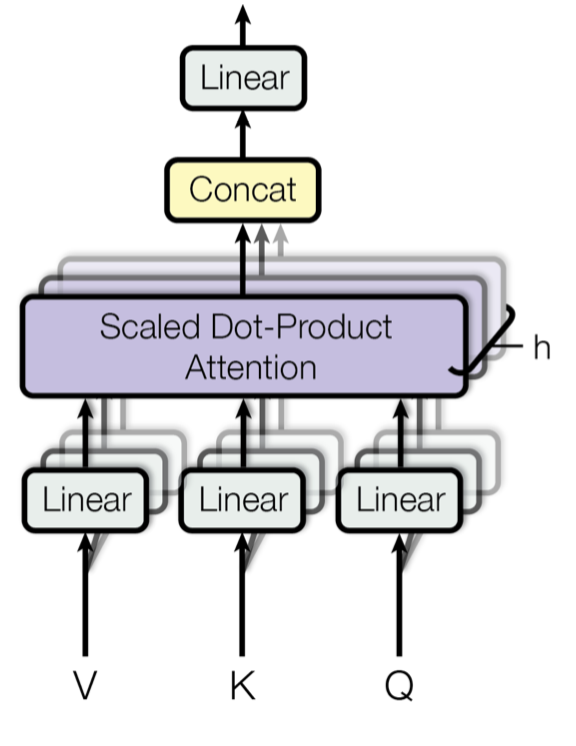
\includegraphics[width=0.5\textwidth]{Figures/appendix/multihead.png}
  \caption{Multi-head attention module as described above. Image source \cite{article:attention}}
  \label{fig:multihead}
\end{figure}

\section{Attention in Graph Attention Networks}\label{sec:attentionGAT}

In their paper \citet{velickovic2017graph} describe a process
of creating a \textit{graph attentional layer}, a process which
is summarized in this section.

The layer takes as input a set of node features, $\bm{h} =
\{\vec{h}_1, \vec{h}_2, \cdots, \vec{h}_N\}, \vec{h}_i \in \mathbb{R^F}$
where $N$ is the number of nodes and $F$ are the features per node.
The output of the layer is a new set of node features (possibly
of differrent cardinality $F'$), $\bm{h'} =
\{\vec{h'}_1, \vec{h'}_2, \cdots, \vec{h'}_N\}, \vec{h}_i'\in\mathbb{R^{F'}}$.

A learnalbe linear transformation is then applied to achieve the required
expressive power to transform the input features to higher-level dimensional
features. This is achieved as a shared linear transformation, parametrized by
a weight matrix $\bm{W} \in \mathbb{R^{F'\times F}}$ and applied to each node.
A shared self-attention $\alpha$ is then applied to all nodes, with $\alpha :
\mathbb{R^{F'}} \times \mathbb{R^{F'}} \rightarrow \mathbb{R}$ which computes
the attentions coefficients:
\begin{equation}
  \label{eq:att_coeff}
  e_{ij} = \alpha (\bm{W}\vec{h}_i, \vec{h}_j)
\end{equation}
which indicates the importance of node $j$'s to node features of node $i$.
Injecting the graph structure in the mechanism (\textit{masked attention})
results in only computing the $e_{ij}$ for $j\in N_i$ where $N_i$ is the neighborhood
of node $i$. A softmax function is then applied to make the coefficients more
easily comparable.

In this implementation, the network is parametrized by a weight vector
$\bm{\vec{a}}^\intercal \in \mathbb{R^{2F'}}$ and a LeakyRELU nonlinearity is applied.
The fully expanded form of this formula is:
\begin{equation}
  \label{eq:full_gan}
  \alpha_{ij}=
  \frac{exp(\text{LeakyRELU}(\bm{\vec{a}}^\intercal[\bm{W}\vec{h}_i\mathbin\Vert\bm{W}\vec{h}_j]))}
  {\sum_{k\in
N_i}
exp(\text{LeakyRELU}(\bm{\vec{a}}^\intercal[\bm{W}\vec{h}_i\mathbin\Vert\bm{W}\vec{h}_k]))}
\end{equation}

where $\mathbin\Vert$ is the concatenation operation.

Finally, after obtaining the normalized attention $\alpha_{ij}$ a linear
combination of the features is obtained and served as the final output
features of each node, after applying a nonlinearity:
\begin{equation}
  \label{eq:final_feature}
  \vec{h}'_i = \sigma \big( \sum_{j\in N_i} \alpha_{ij}\bm{W} \vec{h}_j\big)
\end{equation}

A multi-head attention approach is used for stabilizing the process of self-attention.
For $K$ independent attention mechanisms executing the process described in \eref{eq:final_feature}, the output feature representation is
\begin{equation}
  \label{eq:final_mult}
  \vec{h}'_i = \Big\|^K_{k=1}\sigma\Big( \sum_{j\in N_i}\alpha_{ij}^k \bm{W^k}\vec{h}_j\Big)
\end{equation}

Using the multi-head approach, the output feature vector $\bm{h}'$ consits of
$KF'$ features for each node. If the multi-head attention is performed in the
final prediction layer of the network, averaging is usually applied and nonlinearity
is not applied until then.